\documentclass[a4paper,11pt,fleqn]{scrartcl}%fleqn pour aligner les equations à gauche
\usepackage{../../Styles/Exercice}

\usepackage{multirow}
\newcommand{\chnum}{Chapitre 05}
\newcommand{\chtitle}{Titrages colorimétriques}
\newcommand{\dtype}{Exercices}

\begin{document}
	\maketitle
    \section{Dosage par étalonnage des ions nitrate}
    Les ions nitrate \ce{NO3-} sont un polluant des eeaux : une eau contenant plus de \SI{50}{\mg\per\liter} d'ions nitrate est déclarée non potable. Une solution aqueuse d'ions nitrate est incolore. Une solution aqueuse d'ions nitrate est incolore, mais prend une soloration jaune en présence d'acide phénoldisulfonique.\\
    On dispose d'une solution d'ions nitrate en présence de cet acide, de concentration $c_0 = \SI{1,0E-3}{\mol\per\liter}$. Par dilution, on prépare une échelle de teintes et on mesure les absorbances à \SI{410}{\nm}, dans une cuve de longueur $l = \SI{1,0}{\cm}$. on obtient les résultats suivants.
    \begin{center}
        \begin{tabular}{|c|>{\centering}m{.12\linewidth}|>{\centering}m{.12\linewidth}|>{\centering}m{.12\linewidth}|>{\centering}m{.12\linewidth}|>{\centering\arraybackslash}m{.12\linewidth}|}
            \hline
            $c$ (\unit{\milli\mol\per\liter}) & \num{1,0} & \num{0,75} & \num{0,50} & \num{0,25} & \num{0,10} \\
            \hline
            $A$ & \num{0,95} & \num{0,67} & \num{0,47} & \num{0,23} & \num{0,10} \\
            \hline
        \end{tabular}
    \end{center}
    \begin{enumerate}
        \item Tracer le graphique d'étalonnage et la droite modèle.
        \item Déterminer son coefficient directeur et en déduire le coefficient d'absorption molaire $\epsilon$ de l'espèce absorbante à \SI{410}{\nm}.
        \item Une eau de rivière est testée dans les même conditions : son absorbance est $A = \num{0,85}$. Déterminer sa concentration en ions nitrate.
        \item Cette eau doit-elle être déclarée non potable ?
    \end{enumerate}

    \section{Relation à l'équivalence}
    On considère le titrage de l'éthanol \ce{C2H6O} par les ions dichromate \ce{Cr2O7^2-} en présence d'ions \ce{H+} en excès. L'équation de la réaction est la suivante :
    $$ \ce{2Cr2O7^2- (aq)+ 3C2H6O (aq)+ 16H+ (aq)-> 4Cr^3+(aq) + 3C2H4O2(aq) + 11H2O(l)}$$
    Un élève a tracé le tableau suivant au brouillon.
    \begin{center}
        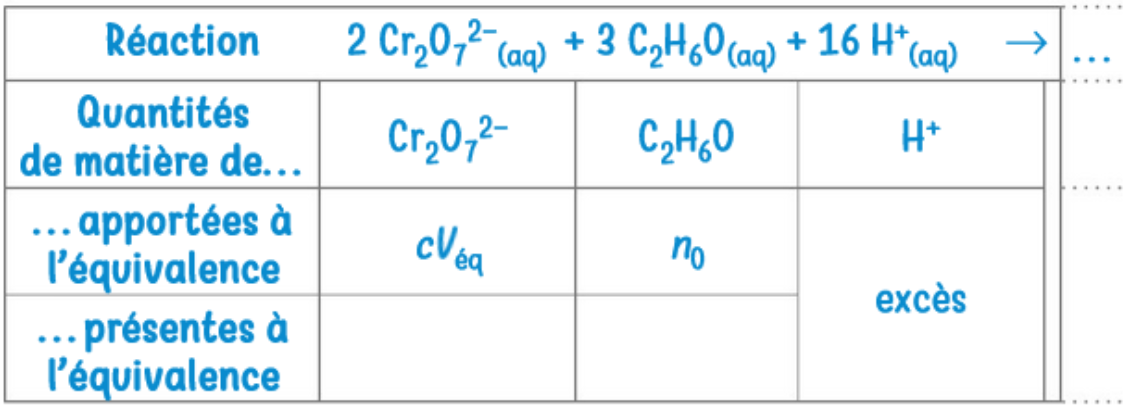
\includegraphics[width = \linewidth]{Ressources/1SPE_C05_Exercice2_tableau.png}
    \end{center}
    \begin{enumerate}
        \item Identifier les notations désignant la quantité de matière d'éthanol introduit, la concentration de la solution titrante et le volume équivalent.
        \item Recopier ce tableau et compléter sa dernière ligne en utilisant la définition de l'équivalence.
        \item En déduire l'expression de la quantité de matière initiale de réactif titré.
    \end{enumerate}

    \section{Titrage et graphiques}
    On reprend le titrage de l'exercice précédent. Le graphique suivant représente les quantités de matière de \ce{Cr2O7^2-}, \ce{C2H6O}, \ce{Cr^3+} et \ce{C2H4O2} dans le mélange réactionnel en fonction du volume $V$ de solution titrante apporté.
    \begin{center}
        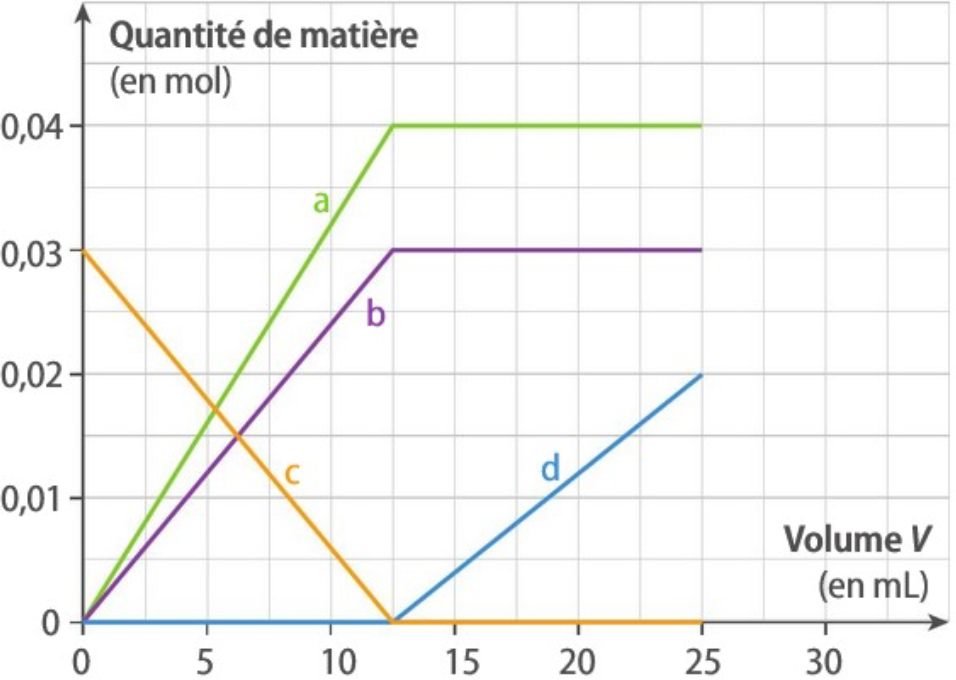
\includegraphics[width = \linewidth]{Ressources/1SPE_C05_Exercice3_graphique.png}
    \end{center}
    \begin{enumerate}
        \item Identifier les courbes correspondant à chaque espèce chimique.
        \item Déterminer le volume équivalent $V_{eq}$, la quantité de matière initiale $n_0$ de réactif titré et la concentration $c$ de la solution titrante.
    \end{enumerate}

    \section{Titrage et incertitudes}
    Lors d'une séance de travaux pratiques, des élèves ont effectué un titrage. les valeurs des volumes équivalents $V_{eq}$ obtenus par les différents groupes eont regroupées ci-dessous.
    \begin{center}
        \begin{tabular}{|c|>{\centering}m{.12\linewidth}|>{\centering}m{.12\linewidth}|>{\centering}m{.12\linewidth}|>{\centering}m{.12\linewidth}|>{\centering\arraybackslash}m{.12\linewidth}|}
    \hline
    \multirow{3}{*}{$V_{eq}$ (\unit{\milli\liter})} & 13,2 & 13,1 & 13,5 & 12,8 & 12,9 \\
    \cline{2-6}
    & 13,0 & 13,2 & 13,3 & 13,2 & 13,0 \\
    \cline{2-6}
    & 12,9 & 13,6 & 13,6 & 13,3 & 13,2 \\
    \hline
\end{tabular}
    \end{center}

\end{document}